\documentclass[12pt]{article}

\usepackage[a4paper,margin=2cm]{geometry}
\usepackage{amsmath}
\usepackage{amssymb}
\usepackage{amsthm}
\usepackage{amsfonts}

\usepackage{algpseudocode}
\usepackage[plain]{algorithm}

\usepackage{caption}
\usepackage{graphicx}
\usepackage{float}
\usepackage{listings}
\usepackage[table]{xcolor}
\usepackage{booktabs}
\usepackage[colorlinks,allcolors=newblue]{hyperref}
\usepackage{microtype}

\usepackage{tikz}
\usepackage[framemethod=TikZ]{mdframed}
\definecolor{newblue}{rgb}{0.2,0.2,0.6}

\usepackage{listings}
\lstset{
    basicstyle=\scriptsize\ttfamily,
    commentstyle=\ttfamily\color{gray},
    numbers=left,
    numberstyle=\ttfamily\color{gray}\footnotesize,
    stepnumber=1,
    numbersep=5pt,
    backgroundcolor=\color{white},
    showspaces=false,
    showstringspaces=false,
    showtabs=false,
    frame=single,
    tabsize=2,
    captionpos=b,
    breaklines=true,
    breakatwhitespace=false,
    title=\ttfamily\lstname,
    escapeinside={},
    keywordstyle={},
    morekeywords={}
}

\newcommand{\handout}[5]{
   \renewcommand{\thepage}{#1-\arabic{page}}
   \noindent
   \begin{center}
   \framebox{
      \vbox{
    \hbox to 5.78in { {\bf ELE 585: Parallel Computing} \hfill #2 }
       \vspace{4mm}
       \hbox to 5.78in { {\Large \hfill #5  \hfill} }
       \vspace{2mm}
       \hbox to 5.78in { {\it #3 \hfill #4} }
      }
   }
   \end{center}
   \vspace*{4mm}
}

\renewcommand{\paragraph}[1]{\medskip \noindent {\bf #1.}}

\newcommand{\lecture}[3]{\handout{#1}{#2}{Professor David Wentzlaff}{By #3}{#1}}

%%%%%% FOUND AT
% https://texblog.org/2015/09/30/fancy-boxes-for-theorem-lemma-and-proof-with-mdframed/

%%%%%%%%%%%%%%%%%%%%%%%%%%%%%%
%Theorem
\newcounter{theo}[section]\setcounter{theo}{0}
\renewcommand{\thetheo}{\arabic{section}.\arabic{theo}}
\newenvironment{theo}[2][]{%
\refstepcounter{theo}%
\ifstrempty{#1}%
{\mdfsetup{%
frametitle={%
\tikz[baseline=(current bounding box.east),outer sep=0pt]
\node[anchor=east,rectangle,fill=blue!20]
{\strut Theorem~\thetheo};}}
}%
{\mdfsetup{%
frametitle={%
\tikz[baseline=(current bounding box.east),outer sep=0pt]
\node[anchor=east,rectangle,fill=blue!20]
{\strut Theorem~\thetheo:~#1};}}%
}%
\mdfsetup{innertopmargin=5pt,innerbottommargin=10pt,linecolor=blue!20,%
linewidth=2pt,topline=true,%
frametitleaboveskip=\dimexpr-\ht\strutbox\relax
}
\begin{mdframed}[]\relax%
\label{#2}}{\end{mdframed}}

%%%%%%%%%%%%%%%%%%%%%%%%%%%%%%
%Proposition
\newcounter{prp}[section]\setcounter{prp}{0}
\renewcommand{\theprp}{\arabic{section}.\arabic{prp}}
\newenvironment{prp}[2][]{%
\refstepcounter{prp}%
\ifstrempty{#1}%
{\mdfsetup{%
frametitle={%
\tikz[baseline=(current bounding box.east),outer sep=0pt]
\node[anchor=east,rectangle,fill=magenta!20]
{\strut Proposition~\theprp};}}
}%
{\mdfsetup{%
frametitle={%
\tikz[baseline=(current bounding box.east),outer sep=0pt]
\node[anchor=east,rectangle,fill=magenta!20]
{\strut Proposition~\theprp:~#1};}}%
}%
\mdfsetup{innertopmargin=5pt,innerbottommargin=10pt,linecolor=magenta!20,%
linewidth=2pt,topline=true,%
frametitleaboveskip=\dimexpr-\ht\strutbox\relax
}
\begin{mdframed}[]\relax%
\label{#2}}{\end{mdframed}}

%%%%%%%%%%%%%%%%%%%%%%%%%%%%%%
%Lemma
\newcounter{lem}[section]\setcounter{lem}{0}
\renewcommand{\thelem}{\arabic{section}.\arabic{lem}}
\newenvironment{lem}[2][]{%
\refstepcounter{lem}%
\ifstrempty{#1}%
{\mdfsetup{%
frametitle={%
\tikz[baseline=(current bounding box.east),outer sep=0pt]
\node[anchor=east,rectangle,fill=green!20]
{\strut Lemma~\thelem};}}
}%
{\mdfsetup{%
frametitle={%
\tikz[baseline=(current bounding box.east),outer sep=0pt]
\node[anchor=east,rectangle,fill=green!20]
{\strut Lemma~\thetheo:~#1};}}%
}%
\mdfsetup{innertopmargin=5pt,innerbottommargin=10pt,linecolor=green!20,%
linewidth=2pt,topline=true,%
frametitleaboveskip=\dimexpr-\ht\strutbox\relax
}
\begin{mdframed}[]\relax%
\label{#2}}{\end{mdframed}}

%%%%%%%%%%%%%%%%%%%%%%%%%%%%%%
%Proof

\newcounter{prf}[section]\setcounter{prf}{0}
\renewcommand{\theprf}{\arabic{section}.\arabic{prf}}
\newenvironment{prf}[2][]{%
\refstepcounter{prf}%
\ifstrempty{#1}%
{\mdfsetup{%
frametitle={%
\tikz[baseline=(current bounding box.east),outer sep=0pt]
\node[anchor=east,rectangle,fill=red!20]
{\strut Proof~\theprf};}}
}%
{\mdfsetup{%
frametitle={%
\tikz[baseline=(current bounding box.east),outer sep=0pt]
\node[anchor=east,rectangle,fill=red!20]
{\strut Proof~\theprf:~#1};}}%
}%
\mdfsetup{innertopmargin=5pt,innerbottommargin=10pt,linecolor=red!20,%
linewidth=2pt,topline=true,%
frametitleaboveskip=\dimexpr-\ht\strutbox\relax
}
\begin{mdframed}[]\relax%
\label{#2}}{\end{mdframed}}

%%%%%%%%%%%%%%%%%%%%%%%%%%%%%%
%Remark
\newcounter{rmk}[section]\setcounter{rmk}{0}
\renewcommand{\thermk}{\arabic{section}.\arabic{rmk}}
\newenvironment{rmk}[2][]{%
\refstepcounter{rmk}%
\ifstrempty{#1}%
{\mdfsetup{%
frametitle={%
\tikz[baseline=(current bounding box.east),outer sep=0pt]
\node[anchor=east,rectangle,fill=yellow!50]
{\strut Remark~\thermk};}}
}%
{\mdfsetup{%
frametitle={%
\tikz[baseline=(current bounding box.east),outer sep=0pt]
\node[anchor=east,rectangle,fill=yellow!50]
{\strut Remark~\thermk:~#1};}}%
}%
\mdfsetup{innertopmargin=5pt,innerbottommargin=10pt,linecolor=yellow!50,%
linewidth=2pt,topline=true,%
frametitleaboveskip=\dimexpr-\ht\strutbox\relax
}
\begin{mdframed}[]\relax%
\label{#2}}{\end{mdframed}}

%%%%%%%%%%%%%%%%%%%%%%%%%%%%%%
%Definiton
\newcounter{dfn}[section]\setcounter{dfn}{0}
\renewcommand{\thedfn}{\arabic{section}.\arabic{dfn}}
\newenvironment{dfn}[2][]{%
\refstepcounter{dfn}%
\ifstrempty{#1}%
{\mdfsetup{%
frametitle={%
\tikz[baseline=(current bounding box.east),outer sep=0pt]
\node[anchor=east,rectangle,fill=cyan!20]
{\strut Definition~\thedfn};}}
}%
{\mdfsetup{%
frametitle={%
\tikz[baseline=(current bounding box.east),outer sep=0pt]
\node[anchor=east,rectangle,fill=cyan!20]
{\strut Definition~\thedfn:~#1};}}%
}%
\mdfsetup{innertopmargin=5pt,innerbottommargin=10pt,linecolor=cyan!20,%
linewidth=2pt,topline=true,%
frametitleaboveskip=\dimexpr-\ht\strutbox\relax
}
\begin{mdframed}[]\relax%
\label{#2}}{\end{mdframed}}

%%%%%%%%%%%%%%%%%%%%%%%%%%%%%%
%Information
\newcounter{info}[section]\setcounter{info}{0}
\renewcommand{\theinfo}{\arabic{section}.\arabic{info}}
\newenvironment{info}[2][]{%
  \refstepcounter{info}%
  \ifstrempty{#1}%
  {\mdfsetup{%
  frametitle={%
  \tikz[baseline=(current bounding box.east),outer sep=0pt]
  \node[anchor=east,rectangle,fill=gray!20]
  {\strut Information~\theinfo};}}
  }%
  {\mdfsetup{%
  frametitle={%
  \tikz[baseline=(current bounding box.east),outer sep=0pt]
  \node[anchor=east,rectangle,fill=gray!20]
  {\strut Information~\theinfo:~#1};}}%
  }%
  \mdfsetup{innertopmargin=5pt,innerbottommargin=10pt,linecolor=gray!20,%
  linewidth=2pt,topline=true,%
  frametitleaboveskip=\dimexpr-\ht\strutbox\relax
  }
  \begin{mdframed}[]\relax%
  \label{#2}
}
{
  \end{mdframed}
}

%%%%%%%%%%%%%%%%%%%%%%%%%%%%%%
%Example
\newcounter{eg}[section]\setcounter{eg}{0}
\renewcommand{\theeg}{\arabic{section}.\arabic{eg}}
\newenvironment{eg}[2][]{%
  \refstepcounter{eg}%
  \ifstrempty{#1}%
  {\mdfsetup{%
  frametitle={%
  \tikz[baseline=(current bounding box.east),outer sep=0pt]
  \node[anchor=east,rectangle,fill=black!20]
  {\strut Example~\theeg};}}
  }%
  {\mdfsetup{%
  frametitle={%
  \tikz[baseline=(current bounding box.east),outer sep=0pt]
  \node[anchor=east,rectangle,fill=black!20]
  {\strut Example~\theeg:~#1};}}%
  }%
  \mdfsetup{innertopmargin=5pt,innerbottommargin=10pt,linecolor=black!20,%
  linewidth=2pt,topline=true,%
  frametitleaboveskip=\dimexpr-\ht\strutbox\relax
  }
  \begin{mdframed}[]\relax%
  \label{#2}
}
{
  \end{mdframed}
}


\definecolor{dfn-color}{rgb}{0,0.48,0.65}

% https://tex.stackexchange.com/questions/227913/meet-and-join-symbols-for-mathematical-lattice-utf-∨-and-∧
\DeclareFontFamily{U}{matha}{\hyphenchar\font45}
\DeclareFontShape{U}{matha}{m}{n}{
      <5> <6> <7> <8> <9> <10> gen * matha
      <10.95> matha10 <12> <14.4> <17.28> <20.74> <24.88> matha12
      }{}
\DeclareSymbolFont{matha}{U}{matha}{m}{n}
\DeclareMathSymbol{\meet}{2}{matha}{"5E}
\DeclareMathSymbol{\join}{2}{matha}{"5F}

\newcommand*{\QED}{\hfill\ensuremath{\square}}
\DeclareMathOperator{\lcm}{lcm}


\begin{document}
\lecture{Class Discussion Notes}{February 11, 2019}{Dev Dabke, Samuel Hsia}

\section{Overview}\label{feb-11:overview}
On this day, we primarily discussed the paper \textit{A View from Berkeley}\cite{Asanovic:EECS-2006-183} (though we also read \textit{Classical Iterative Methods for Systems of Linear Equations} from \textit{Parallel and Distributed Computation: Numerical Methods}\cite{Bertsekas:1989:PDC:59912}, this paper will be discussed at a future date).

\section{A View from Berkeley}\label{feb-11:a-view}
\subsection{Paper Overview}\label{feb-11:a-view:overview}
According to our class, this paper is about
\begin{itemize}
    \item Everything about parallel computing
    \item The state of the art (in 2006) and how we should transform the field
\end{itemize}
This paper is authored by researchers and scientists from various fields (e.g.\ computer architecture, scientific computing, etc).
They are mostly faculty or senior research scientists at UC Berkeley (at the time, Krste Asanovic was moving from MIT to UCB).

Additionally, we determined that, stylistically, this paper:
\begin{itemize}
    \item Is a summary of these researchers' discussions on parallel computing
    \item A technical report
    \item A position paper
    \item Tried to lay down a roadmap of how they expect people should develop parallel programs, systems, and architectures
    \item Has a lot of strong positions
    \item Has positions based on reasoning, rather than empirical evidence (e.g.\ the argument a move from multicore to manycore is necessary)
\end{itemize}

\subsection{Primary Contribution}\label{feb-11:a-view:contribution}
Some ideas for this paper's primary contribution were:
\begin{itemize}
    \item Setting standards for evaluating parallel computing
    \item Providing guidelines for designing parallel computing systems
    \item The new conventional wisdoms
    \item The dwarfs (i.e.\ high-level abstraction over measuring performance for parallel computing)
    \item The potential benefits of a human-centric approach for designing future parallel computing systems (i.e.\ systems in which the exposed software has a lot more potential for performance gains).
    \item Though it has many contributions, this paper provides the most comprehensive synthesis and analysis of the best available relevant information at the time
\end{itemize}

\subsection{Key Insights}\label{feb-11:a-view:insights}

We also enumerated what some of the key insights were
\begin{enumerate}
    \item Manycore will beat multicore
    \item The dwarfs (i.e.\ high-level abstraction over measuring performance for parallel computing)
    \item The new conventional wisdoms
    \item The potpourri of ancillary considerations (autotuners, architectural suggestions)
    \item That smaller/simpler is better: deep pipelines don't help parallelism (e.g.\ Intel Tejas processor, internally the Pentium 8, hit the \textit{power wall} and was cancelled because of power considerations)~\cite{Tejas}.
\end{enumerate}

\subsection{Manycore vs.\ Multcore}\label{feb-11:a-view:many-vs-multi}
As an aside, we also discussed the difference between manycore and multicore, since these terms were used---but not explicitly defined---in the paper. The following table summarizes some of the more notable characteristics for manycore and multicore computer systems.

\rowcolors{2}{gray!25}{white}
\begin{center}
    \begin{tabular}{p{5cm} p{5cm} p{5cm}}
        \toprule
        & Manycore & Multicore \\
        \midrule
        Interconnect Network & Bus & No C \\
        \# of Cores & \( <10 \) & \( >10 \) \\
        Design Methodology & Uses uniprocessors as building blocks & Designed from the ground up to handle a large number of cores (up to \( 1000 \)s range); contains other things you add into the system that facilitate parallel computing \\
        \bottomrule
    \end{tabular}
\end{center}

\subsection{Like and Dislike}\label{feb-11:a-view:like-dislike}
We also discussed what everyone liked and disliked about this paper:

\textbf{Likes:}

\begin{itemize}
    \item High level update of conventional wisdoms, i.e.\ the changes in how people viewed computer systems;
    \item Tensions between embedded (even predates the first iPhone, which was released in 2007) and HPC
    \item How architecture improvements should be exposed to software system developers in order to realize full potential of parallelism
    \item Very comprehensive, great to see parts (i.e.\ suggestions and possible solutions) that computer systems engineers should consider during the design process.
    \item High level view on what should be solved in parallel computing systems and understanding how the different fields interact with each other
    \item Systematic organization
    \item Dwarfs are a huge approach to try to summarize computational patterns and also help us in our design process
    \item Don't agree that they push their research agendas, since they have to propose something.
    Their ideas can be used as starting points/suggestions for future designs.
\end{itemize}

\noindent \textbf{Dislikes:}

\begin{itemize}
    \item Decent amount of technical expertise required to appreciate the paper, as seen in the list of authors (experts in computer architecture, supercomputing, compilers, algorithms, etc.)
    \item General vagueness in the discussion on human factors in productivity (i.e.\ ``research in human factors research leads to higher productivity'')
    \item Paper is very opinionated and leaves little room for discussion
    \item Unstated assumptions (i.e. Silicon dominance)
    \item Drastic differences in how we perceive manycores then and now.
    \item Missclassification of GPUs: While our general purpose computers do not have cores that scale into the thousands range, we now consider GPUs to be a form of manycore processors (multiple shader processing units). Interestingly, this papertalks about Cg, which predates CUDA (used by rocket scientists/ supercomputing people).
    \item Optimism/pessimism about certain things
    \item The paper is actively not discussing specialization, more on parallelization.
    \item Lots of stating general computer architecture design guidelines without explanation.
    \item Pushing of own research agendas

\end{itemize}

\subsection{Conventional Wisdom}\label{feb-11:a-view:conventional}
In some sense, this paper, in its view of the Golden Gate Bridge from UC Berkeley, is trying to give something to every researcher.
This paper thus introduces some ``conventional wisdom.''
We discuss how this ``wisdom'' has or has not held up, and if it was even true at the time.

\begin{enumerate}
    \item Not true: Power Wall. Transistors are no longer really ``free;''  we are sort of stuck at 7nm without significant device innovations that can save the day.
    \item Not true: Leakage solved by device innovations (i.e.\ FinFET)
    \item True: errors definitely got worse
    \item True: constraints become more important as you shrink feature size
    \item Not really true: RAMP never really took off. However, more sophisticated FPGAs have allowed for an alternative test platform
    \item Kind of true: starting to see problems with bandwidth, but latency is still an issue
    \item old CW not even true then: Memory Wall is still a problem
    \item True
    \item True
    \item True
    \item True
    \item True for some applications but less so; more emphasis on other costs
\end{enumerate}

\subsection{The Dwarfs}\label{feb-11:a-view:dwarfs}

This paper also introduces a notion of \textit{dwarfs}.
Although this paper is not the first to use this terminology, they co-opted and extended it for the purposes of parallel computing.

We postulated a few definitions for a dwarf:
\begin{itemize}
    \item better word: ``kernel''
    \item a testing program
    \item a benchmark
    \item an application domain
\end{itemize}
We converged on these distinctions:
\begin{enumerate}
    \item A \textit{dwarf} is a general application domain that is not actionable, e.g.\ Spectral Methods
    \item A \textit{kernel} is a specific problem or algorithm within a dwarf, e.g.\ FFT
    \item A \textit{benchmark} is a specific implementation of a kernel, e.g.\ a specific program that runs FFT
\end{enumerate}
We also debated if dwarfs were useful:

While dwarfs lack the specificity of kernels and benchmarks, they can often be used as a guiding direction for designing systems for applications dominated by a single or set of kernels.
Understanding the dwarves can also help us create better benchmarks: perhaps when implementing a benchmark, tracking a dwarf to get a general gist of its performance requirements would be useful.

However, it's important to note that whereas kernels and benchmarks are actionable, dwarfs are not.
This leads to the major drawback of inability for comparison (i.e.\ how do you compare a GPU against a manycore?).

There was also a discussion on the conciseness of the list of dwarves and we generally agreed that the \textit{Monte Carlo} dwarf and some of the ones added later on were either too general or too problem-specific.

\subsubsection{Usefulness/Communication patterns of Dwarfs}

\begin{enumerate}
    \item Dense LA:\ probably useful; while can't map all small neighborhoods next to each other the communication pattern is generally localized
    \item Sparse LA:\ localization, but further communication as well
    \item Spectral Methods (i.e.\ FFT, real/complex-valued):\ communication from everybody to everybody; not as bad as \( n \)-body, as there is some structure (Figure~\ref{fig:butterfly}).
    \item \( n \)-body problem: if we zoom in on this communication pattern, we don't see that everything communicates.
    The communication pattern is an approximated \( n \)-body with neighborhoods; good approximation for certain applications, but not for others.
    \item Structured Grids: some PDE solvers
    \item Unstructured Grids: graph computations
    \item Monte Carlo (clumped with other embarrassingly parallel application, probably not the best idea)
\end{enumerate}

\begin{figure}
    \centering
    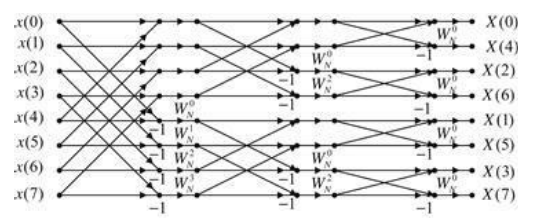
\includegraphics[width = 0.8\linewidth]{fig/butterfly}
    \caption{Butterfly diagram for an eight-point FFT (total 12 multiplications)~\cite{DSP_Tan}}\label{fig:butterfly}
\end{figure}

\bibliography{citation}{}
\bibliographystyle{alpha}

\end{document}
